
\documentclass[9.5pt]{extarticle}

\usepackage{full page}  % make the margins somewhat smaller than the default
\usepackage{graphicx}
\usepackage{amsmath}
\usepackage{indentfirst}
\usepackage{color}
\usepackage{cite}
\usepackage{wasysym}
\usepackage{amssymb}
\usepackage{multirow}
\usepackage{float}
\usepackage{lscape}
\usepackage{alltt} 
\usepackage{listings}
\usepackage{booktabs}
\usepackage{mathtools}
\usepackage{fancyhdr}
\usepackage[table,xcdraw]{xcolor}

\DeclarePairedDelimiter{\ceil}{\lceil}{\rceil}
\DeclarePairedDelimiter{\floor}{\lfloor}{\rfloor}

\definecolor{dkgreen}{rgb}{0,0.6,0}
\definecolor{gray}{rgb}{0.5,0.5,0.5}
\definecolor{mauve}{rgb}{0.58,0,0.82}


\usepackage{listings}  %  needed for source code listings

\lstset{frame=tb,
  language= java,
  aboveskip=1.5mm,
  belowskip=1.5mm,
  showstringspaces=false,
  columns=flexible,
  basicstyle={\small\ttfamily},
  keywordstyle=\color{blue},
  commentstyle=\color{dkgreen},
  stringstyle=\color{mauve},
  breaklines=true,
  tabsize=2,
  numbers=left,
  stepnumber=1,    
  firstnumber=1,
  numberfirstline=true
}
       

% set the document title, author, and date here.
%  once set, the \maketitle command (within the document)
%  will display them nicely
\title{CS3243 Group 25 Project 2: Sudoku Solver using Backtracking Search}
\author{Choong Jin Yao (A0173247A), Dominic Frank Quek (A0173261L),\\ Yang Shuqi (A0177383U), Yang Yiqing (A0161424A)}

\begin{document}
\maketitle

\section{Introduction}
Constraint Satisfaction Problem (CSP) search algorithm uses the structure of states and a general purpose heuristic to solve problems. We are given the task of implementing a Sudoku solver using backtracking algorithm with relevant heuristics. 

\section{Problem Specification}
The puzzle is modeled as a list of 81 cells where each cell is represented by an (x, y) coordinate where $ 1\leq \verb`x,y` \leq 9$. Every cell is assigned a value \verb`v` where  $ 0\leq \verb`v` \leq 9$. An empty cell is where $v = 0$. The variables are the coordinates of empty cells in the given input puzzle. A list \verb`unassigned_var_list` contains the variables that are yet to be assigned a value. The constraints are that for any of the 9 rows, 9 columns and 9 diagonals, no value can appear more than once. To enforce this constraint, at the start, we initialise 27 lists containing the legal values for each row, column and diagonal after removing the pre-assigned values in the given input puzzle. Then, we keep track of the domain of each variable where the domain contains the legal values to be assigned to that variable. The domains are updated to be consistent with the 27 lists. 

Afterwards, we begin the backtracking search algorithm. When a value is assigned to a variable, the variable is removed from \verb`unassigned_var_list` and its domain becomes empty. After every assignment, we use heuristics to remove illegal values from the domains of neighbouring variables. Hence, the constraints are guaranteed not to be violated throughout.

\section{Algorithm variants}
We implemented a backtracking solver that incorporates these variants: 

\indent \indent 1) Variable ordering: choosing the most constrained variable with Minimum Remaining Values (MRV) \indent \indent heuristic with/without tie-breaking with Degree heuristic

\indent \indent 2) Value ordering: Least Constraining Value (LCV) heuristic 

\indent \indent 3) Inference: Forward Checking or Arc Consistency-3(AC3) .  

After implementation, we evaluate and select the best variant from the timinig gathered from the \indent heuristics on the Sudoku problem. 

\subsection{Backtracking}

Backtracking is a recursive search algorithm that allows for reversion of value assignments when a certain complete assignment turns out to be unsuccessful. When that occurs, we restore the domains prior to the assignment to the variable. It recurses if the assigned variable is consistent with its neighbouring constraints.  The backtracking algorithm forms the backbone of the entire search as seen in the function \verb`backtracking_search`. Within the backtracking algorithm, heuristics are implemented in 3 aspects: Variable Ordering, Value Ordering and Inference.

\subsection{Variable Ordering}
We prioritized the variable for expansion that is the most constrained. For this, we experimented with 2 heuristics: Minimum Remaining Value (MRV) and Degree.

\subsubsection{Most Constrained Variable: Minimum Remaining Value}

Minimum Remaining Value chooses the variable with the least number of legal values. This is basically the variable with the smallest domain size. Note that when the domain size of an unassigned variable is 0, the assignment is impossible and the algorithm will backtrack. MRV is implemented in the function \verb`minimum_remaining_values`.

\subsubsection{Most Constraining Variable: Degree}
Degree heuristic acts as a tie-breaker among the Most Constrained Variable using MRV heuristic. Among variables that have least and equal domain sizes, the variable with the most unassigned neighbours is prioritized. By doing this, it potentially further reduces the search space as it leads to a maximal reduction in domains for other variables. Degree heuristic is implemented in the function \verb`degree`. 

\subsection{Value Ordering: Least Constraining Value}

Least Constraining Value heuristic prioritizes the domain value of a variable that results in the minimum reduction in the domains of neighbouring variables. In our implementation, we count the number of conflicts between the value and the values of its neighbours. A conflict simply happens when the value of the target variable is contained in the domain of a neighbouring variable. The value with the least number of conflicts is then prioritized. LCV is implemented in the function \verb`least_constraining_value` that sorts the variable domain using the \verb`count_conflicts` function as the key.


\subsection{Inference}

Inference is effective in reducing the domain of variables hence significantly reducing search space. Whenever a value is assigned to a variable, we can infer new domain reductions on its neighbouring variables. We have experimented with 2 variants: Forward Checking (FC) and Arc Consistency (AC-3). 


\subsubsection{Forward Checking}

Forward Checking ensures that a value assignment is consistent with the domains of all its neighbouring variables. Fundamentally, it ensures that the assigned variable is arc-consistent with the other variables. FC prunes the the domain values of variables that are in conflict with the value assignment. Failure is detected when any of the reduced domains is empty as a result. This is implemented in the function \verb`forward_checking`.

\subsubsection{AC-3}

Whereas FC ensures arc consistency between a certain variable and the other variables, AC-3 ensures arc consistency between any 2 variables after every value assignment. This requires an initilisation of binary constraints where we create a tuple for each pair of neighbour variables as seen in the function \verb`init_binary_constraints`. After every assignment, we loop through the list of binary constraints, reducing the domains whenever necessary. Whenever a domain is reduced using the \verb`revise` function, the binary constraints of the neighbours are added to the queue. Evidently, this can be computationally expensive. This is implemented in the function  \verb`ac_3` and the subfunction \verb`revise`. 

\section{Experimental Setup}

For the experimental setup, we run different variants of the aforementioned heuristics. We measure the perfomance of each variant by measuring the running time. Measuring the runtime allows us to compare the efficiency of the variants in terms of time. The runtime of the variant covers all the work done and computations by the involved heuristics.

We find it inaccurate and difficult to measure and compare the search space of different variants via computing the number of traversed nodes. It is impossible to establish a fair definition of what a node represents. This is due to the different implementations of various heuristics. For instance, for AC-3, on top of the number of value assignments made before arriving at a solution, it also requires checking through every binary constraint everytime an assignment occurs. For FC,  it requires traversing the domains of remaining unassigned variables. We can simply define it to be the number of assignments made (equivalently, the number of calls to the \verb`recursive_backtrack` function. However, that is clearly too trivial and inaccurate as the additional work done outside by the heurstic is not accounted for. 

Additionally, we test the variants on the world's hardest Sudoku puzzle that we've found online (Taken from https://www.conceptispuzzles.com/index.aspx?uri=info/article/424).

\begin{figure}[H]
\centering
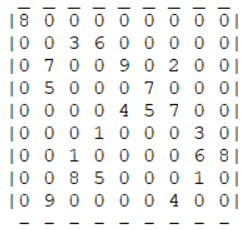
\includegraphics[scale=0.9]{hardest_sudoku.png}
\caption{World's Hardest Sudoku}
\label{Figure 1}
\end{figure}

\section{Results and Discussion}

 The results for runtime performance is given in Table 1, number of nodes explored is given in Table 2. Note that for runtimes that are larger than 300 seconds, we put a '-' symbol.\\

As can be observed from Table 1, FC+MRV+ LCV has the fastest overall run time for the sudoku problem, even though it is slower than AC3+MRV+LCV for input 1. This could be due to the uniqueness of input 1. It also seems like LCV, instead of speeding things up, actually slow things down. A possible explanation is the sorting algorithm used in \verb`orderDomainValues` introduced a \verb`nlog(n)` factor to the runtime, thus slowing things down. FC might be faster than AC-3 because it tracks fewer nodes when checking for consistency. In addition, if there is an inconsistency caused by an assigned variable, usually it will be detected near the assigned variable instead of further away. It is interesting to note that the hard sudoku problem can only be solved within a minute when there is FC or MRV with AC-3 heuristic involved. It is also interesting to note that the number of nodes explored is the least for FC+MRV. Again, FC and MRV reduces the number of node explored while LCV increases the number of nodes explored. Therefore, overall FC and MRV gives the greatest improvement in runtime. If the\\

\begin{table}[H]
\resizebox{\textwidth}{!}{%
\begin{tabular}{@{}rccccccccccc@{}}
\toprule
Run time (seconds)   & MRV  & FC   & FC+LCV  & FC+MRV   & FC+MRV+LCV      & MRV+LCV & AC3     & AC3+MRV+LCV & AC3+MRV & AC3+LCV\\ \midrule
Sudoku (input1)        & 0.07 &-        & -           & 0.915    & 0.347                  & -                  & -         & 0.251            & 0.612 &-       \\
Sudoku (input2)        & -      &9.311 & 0.093    &0.013      &0.003                & 17.46              & 0.141    & 0.015           & 0.023 & 0.030     \\  
Sudoku (input3)        & 0.07& 0.109 & 0.142   &0.002     & 0.002              & 0.31                 & 0.023   & 0.023            & 0.023 & 0.023      \\
Sudoku (input4)        & -      & 0.357 &0.925  &0.003       &0.003                & 17.46               & 0.024    & 0.016           & 0.011 & 0.018     \\ 
Sudoku (hardest)      &       &           &          &            & \\
\bottomrule
\end{tabular}
}
\centering
\caption{Experiments performed to measure runtime with various heuristic on Sunfire}
\label{my-label}
\end{table}

\section{Conclusion}










\end{document}